\documentclass{standalone}
\usepackage{tikz}
\usepackage{ctex,siunitx,bm}
\usepackage{tkz-euclide}
\usepackage{amsmath,mhchem}
\usetikzlibrary{patterns, calc}
\usetikzlibrary {decorations.pathmorphing, decorations.pathreplacing, decorations.shapes,}
\begin{document}
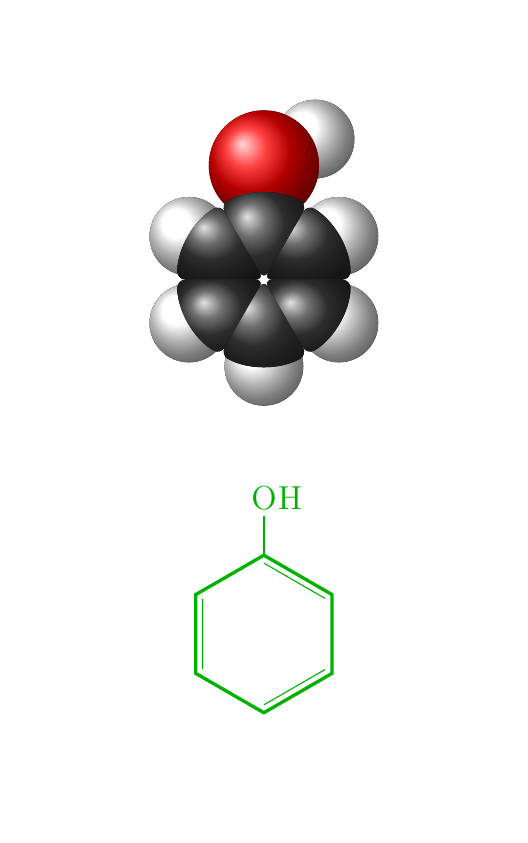
\begin{tikzpicture}[scale=1.0]
  \useasboundingbox(-3,3.2)rectangle(3,-6.8);
  \begin{scope}[scale=1]
  \fill[ball color=white](70:1.9)circle(0.5);
  \fill[ball color=red](90:1.45)circle(0.7);
  \foreach \x in {30,150,210,270,330}
  {
    \fill[ball color=white](\x:1.1)circle(0.5);
    \fill[ball color=darkgray,rounded corners=3pt](0,0)--(\x-30:1.1)arc(\x-30:\x+30:1.1)--cycle;
  }
  \fill[ball color=darkgray,rounded corners=3pt](0,0)--(60:1.1)arc(60:120:1.1)--cycle;
  \end{scope}
  \begin{scope}[yshift=-4.5cm]
    \draw[very thick,green!70!black](30:1)--(90:1)--(150:1)--(210:1)--(270:1)--(330:1)--cycle;
    \draw[thin,green!70!black](150:0.9)--(210:0.9)(270:0.9)--(330:0.9)(30:0.9)--(90:0.9);
    \draw[semithick,green!70!black](90:1)--++(0,0.5)node(O)[above=2pt,inner sep=0pt]{\large\ce{O}};
    \node at (O.east)[right,inner sep=0pt,green!70!black]{\large\ce{H}};
  \end{scope}
\end{tikzpicture}
\end{document}